\chapter{Field Theory}
\label{sec:field_theory}
In the last sections, we dealt with discrete and finite dimensional problems. Now, we want to extend our theory to an infinite number of degrees of freedom and apply it on field theory. The main difference is that we can analyse not only several points but every point in space at once. Imagine assigning the amplitude $q(\bar{x})$ to each point $\bar{x} \in \mathbb{R}^3$:

\begin{example}  
\begin{align}
L(q_i,\dot{q}_i) = \sum_{i=1}^n \left( \frac{\dot{q}_i^2}{2} - \gamma \frac{q_i^2}{2} \right).
\end{align}
In the finite dimensional case, we just have n oscillating points. 
\begin{align}
L[q_{\bar{x}},\dot{q}_{\bar{x}}] = \int d^3 x \left( \frac{\dot{q}^2(\bar{x})}{2} - \gamma \frac{q^2(\bar{x})}{2} \right).
\end{align}
Now, we have oscillators in every point of space.
\end{example}

In field theory, for instance, we want to know the value of the field $\varphi$ in every point $\bar{x}$, see Fig.~\ref{fig:6}. Of course, there is the option to assign more than one field to every point $\bar{x}$.
One can see that the discrete index $i$ is replaced by the continous variable $\bar{x}$.

\begin{figure}[H]
\begin{center}
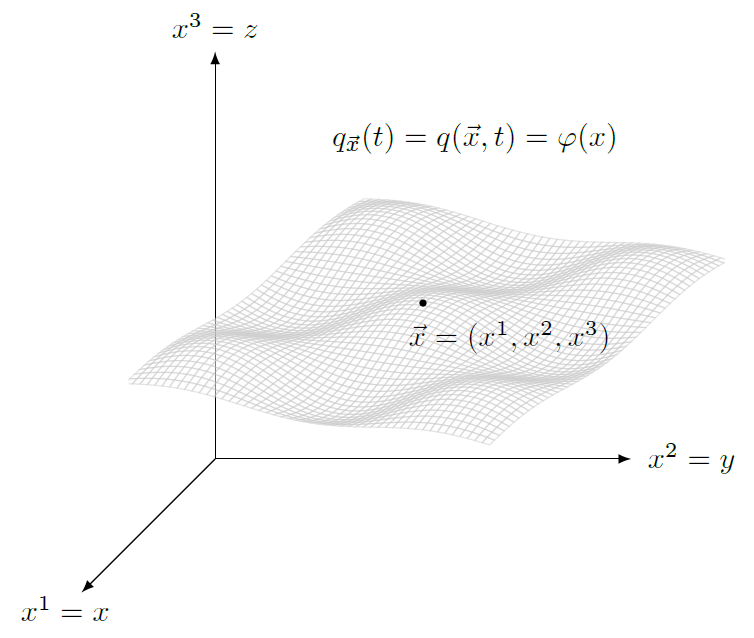
\includegraphics[scale=0.7]{img/field.png}
\end{center}
\caption{Assigning the value of the field $\varphi$ to each point $\bar{x} \in \mathbb{R}^3$.}
\label{fig:6}
\end{figure}

The difference between finite dimensional and infinite dimensional theory is summerized in the following table: 

\begin{table}[H]
\begin{tabular}{>{\centering}p{.45\textwidth} | >{\centering}p{.45\textwidth}} 
Discrete case \vspace{5pt} & Continuous case \vspace{5pt} \tabularnewline \hline 
\vspace{5pt} $q_i(t), \ \ \ i=1, \dots, n$ & \vspace{5pt} $q_{\bar{x}}(t) = q(\bar{x},t), \ \ \ \bar{x} \in \mathbb{R}^3$ \tabularnewline 
\vspace{3pt} $\sum_{i=1}^n$ & \vspace{3pt} $\int d^3 x$ \tabularnewline 
\vspace{3pt} $L(q_1, \dots, q_n, \dot{q}_1, \dots, \dot{q}_n)$ & \vspace{3pt} $L[q_{\bar{x}}, \dot{q}_{\bar{x}}]$ \tabularnewline 
\end{tabular}
\caption{Comparison between finite dimensional and infinite dimensional theory.}
\end{table}

We want our theory to be relativistic invariant, so we have to make our fields dependent on time $q(t, \vec{x}) = q(x^{\mu})$ and build the Lagrangian out of Lorentz scalars:
\begin{align}
L = \frac{1}{2} \int d^3 x \left( \dot{q}^2 - \gamma q^2 \right) \ \ \longrightarrow \ \ \frac{1}{2} \int d^3 x \left( \partial_{\mu} q \partial^{\mu} q - \gamma q^2 \right),
\end{align}
where $\mu = 0,1,2,3$. If we apply a Lorentz transformation on the old Lagrangian, space and time are mixed together so that we get a different result. The new Lagrangian should be build in a way to compensate this mixing and leave the action invariant under Lorentz transformations. We will use the $(+ - - -)$ signature of Minkowski spacetime. \\
The simplest example for such a relativistic invariant field theory is the Klein-Gordon-Fock field:

\begin{example}[Klein-Gordon-Fock field]
\begin{align}
L[\varphi, \dot{\varphi}] &= \frac{1}{2} \int d^3 x \left( \partial_{\mu} \varphi \partial^{\mu} \varphi - m^2 \varphi^2 \right) \notag \\
&= \frac{1}{2} \int d^3 x \left( \dot{\varphi}^2 - (\nabla \varphi)^2 - m^2 \varphi^2 \right) \notag \\
&= \frac{1}{2} \int d^3 x \left( \dot{\varphi}^2 + \varphi \Delta \varphi - m^2 \varphi^2 \right) \notag \\
&= \frac{1}{2} \int d^3 x \left( \dot{\varphi}^2 + \varphi (\Delta - m^2) \varphi \right).
\end{align}
This Lagrangian is regular, so no constraints appear.
\end{example}

We would like to illustrate the Hamiltonian formulation of field theory with the KGF field. The above form of the Lagrangian will be useful later. \\
The next step is to find the Hamiltonian from a given Lagrangian. In the discrete case, we used to differentiate the Lagrangian with respect to the generalized velocities to find the conjugated momenta. What are the generalized velocities now and how to define the conjugated momenta in field theory? To answer this questions, we will need a mathematical tool which we want to develop in the next section. 

\pagebreak

\section{Functional derivative}

The directional derivative for a function $M(q_1, \dots, q_n)$ of $n$ varibles is defined as
\begin{align}
\frac{\partial M}{\partial q_k} = \lim_{a \rightarrow 0} \ \frac{M(q_1, \dots, q_k + a, \dots, q_n) - M(q_1, \dots, q_k, \dots, q_n)}{a}.
\end{align}
We want to generalize the directional derivative for functionals
\begin{align}
M(q_1, \dots, q_n) \ \longrightarrow \ M[q(x)].
\end{align}
The problem is that the functional doesn't depend on the variable $x$ but on the function $q$. For instance, if $x \in [a,b]$, we have to consider every possible path from $a$ to $b$:
\begin{figure}[H]
\begin{center}
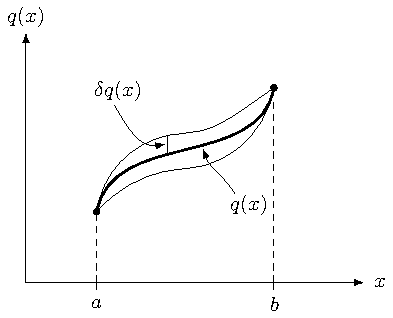
\includegraphics[scale=1.8]{img/variation.pdf}
\end{center}
\caption{Variation of a path $q(x)$ with fixed endpoints.}
\label{fig:7}
\end{figure}
Usually, the knowledge of the complete functional for all possible paths is not required. We rather want to know the behavior of the functional in the vicinity of the function $q$, which makes it extremal or stationary. Therefore, we can take the path $q(x)$ and disturb or variate it by adding a small but arbitrary function $\delta q(x)$. One way of generalizing the directional derivative is by using the variation $\delta M$ of the functional $M[q(x)]$:

\begin{definition}[Functional derivative]
\begin{align}
\delta M \equiv M[q(x) + \delta q(x)] - M[q(x)] = \displaystyle\int\limits_{a}^{b} dx \ \frac{\delta M[q]}{\delta q(x)} \ \delta q(x).
\end{align}
\end{definition}

\pagebreak

If we write $\delta q(x) = \varepsilon \ \eta(x)$, where $\eta(x)$ is an arbitrary function and $\varepsilon$ is infinitesimally small, we can Taylor expand our definition and find:
\begin{align}
\left. \frac{d M[q + \varepsilon \eta]}{d\varepsilon} \ \right|_{\varepsilon=0} = \displaystyle\int\limits_{a}^{b} dx \ \frac{\delta M[q]}{\delta q(x)} \ \eta(x).
\end{align}

This is a useful result to calculate the functional derivative, if one has more complicated functionals. Now, let us look at some simple examples to get comfortable with the definition and understand what's going on.
\vspace{15pt}
\begin{example}
Consider the following functional
\begin{align}
M[q(x)] =  \displaystyle\int\limits_{a}^{b} dx \ q(x).
\end{align}
We can use our definition of the functional derivative
\begin{align}
\delta M = \displaystyle\int\limits_{a}^{b} dx \left( q(x) + \delta q(x) \right) - \displaystyle\int\limits_{a}^{b} dx \ q(x) = \displaystyle\int\limits_{a}^{b} dx \ \delta q(x) \overset{!}{=} \displaystyle\int\limits_{a}^{b} dx \ \frac{\delta M}{\delta q(x)} \ \delta q(x)
\end{align}
and read off the result
\begin{align}
\frac{\delta M}{\delta q(x)} = 1.
\end{align}
\end{example}
\vspace{20pt}
\begin{example}
Next, let us take the functional
\begin{align}
K[q(x)] =  \displaystyle\int\limits_{a}^{b} dx \ q^n(x).
\end{align}
Then, we can use our helpful result
\begin{align}
\left. \frac{d K[q + \varepsilon \eta]}{d\varepsilon} \ \right|_{\varepsilon=0} = \displaystyle\int\limits_{a}^{b} dx \ n q^{n-1}(x) \ \eta(x) \overset{!}{=} \displaystyle\int\limits_{a}^{b} dx \ \frac{\delta K}{\delta q(x)} \ \eta(x) 
\end{align}
to find
\begin{align}
\frac{\delta K}{\delta q(x)} = n q^{n-1}(x).
\end{align}
\end{example}
\vspace{15pt}


One can see that the functional derivative is very similar to the ordinary derivative. In fact, all the properties of the ordinary derivative (like Leibniz rule, chain rule, ...) are satisfied by the functional derivative. We want to show one last useful tool for working with functional derivatives. It is no coincidence that the functional derivative of the above examples looks like the ordinary derivative. \\


More general, we have the property that
\begin{align}
M[q(x)] = \displaystyle\int\limits_{a}^{b} dx \ f(q(x)) \ \ \Longrightarrow \ \ \frac{\delta M}{\delta q(y)} = f'(q(y)).
\end{align}

\begin{proof}
Consider a parametrized family of functionals $M_z[q(x)]$. For a fixed $q$, we can have different outputs depending on $z$. So it looks much like a function with variable $z$:
\begin{align}
M_z[q(x)] \equiv q(z).
\end{align}
By calculating the variation
\begin{align}
\delta M_z &= M_z[q(x) + \delta q(x)] - M_z[q(x)] = q(z) + \delta q(z) - q(z) = \delta q(z) \notag \\
&= \displaystyle\int\limits_{a}^{b} dx \ \delta(x-z) \delta q(x).
\end{align}
we note that 
\begin{align}
\frac{\delta q(z)}{\delta q(x)} \equiv \frac{\delta M_z}{\delta q(x)} = \delta(x-z).
\end{align}
With a bit more work, one can show some more properties of the functional derivative (like changing the order of integration and derivation or the chain rule) and get
\begin{align}
\frac{\delta M}{\delta q(y)} = \displaystyle\int\limits_{a}^{b} dx \ \frac{\delta f(q(x))}{\delta q(y)} = \displaystyle\int\limits_{a}^{b} dx \ f'(q(x)) \frac{\delta q(x)}{\delta q(y)} = f'(q(y)). 
\end{align}
\end{proof}



\section{Hamiltonian description}

Now, we are in the position to continue with the Hamiltonian description of field theory. First, we will define the needed quantities in general and see how the Hamiltonian equations generalizes in field theory. After, we will apply it to the KGF field and see how to interpret the results. Let's go ahead and define the conjugated or generalized momentum for a given field $\varphi$ to be:

\begin{definition}[Generalized momentum]
\begin{align}
\pi(\bar{x}) = \frac{\delta L}{\delta \dot{\varphi}(\bar{x})}.
\end{align}
\end{definition}

The Hamiltonian will be given by
\begin{definition}[Hamiltonian]
\begin{align}
H[\varphi(\bar{x}), \pi(\bar{x})] = \int d^3 x \ \dot{\varphi}(\bar{x}) \pi(\bar{x}) \ - \ L.
\end{align}
\end{definition}


The equation of motion (or time-evolution) is calculated like before
\begin{align}
\dot{g}[\varphi(\bar{x}), \pi(\bar{x})] = \left\{ g,H \right\},
\end{align}
where the Poisson bracket is defined analogous to the discrete case by
\begin{definition}[Poisson bracket]
\begin{align}
\left\{ f,g \right\} \equiv \displaystyle\int d^3 z \left( \frac{\delta f}{\delta \varphi(\bar{z})} \frac{\delta g}{\delta \pi(\bar{z})} - \frac{\delta g}{\delta \varphi(\bar{z})} \frac{\delta f}{\delta \pi(\bar{z})} \right).
\end{align}
\end{definition}

The Hamiltonian equations of motion in field theory take the form:
\begin{align}
\dot{\varphi}(\bar{x}) = \left\{ \varphi(\bar{x}),H \right\} = \displaystyle\int d^3 z \ \frac{\delta \varphi(\bar{x})}{\delta \varphi(\bar{z})} \frac{\delta H}{\delta \pi(\bar{z})} &= \displaystyle\int d^3 z \ \delta^3(\bar{x} - \bar{z}) \frac{\delta H}{\delta \pi(\bar{z})} = \frac{\delta H}{\delta \pi(\bar{x})} \\
\dot{\pi}(\bar{x}) = \left\{ \pi(\bar{x}),H \right\} = - \displaystyle\int d^3 z \frac{\delta H}{\delta \varphi(\bar{z})} \frac{\delta \pi(\bar{x})}{\delta \pi(\bar{z})} &= - \displaystyle\int d^3 z \frac{\delta H}{\delta \varphi(\bar{z})} \delta^3(\bar{x} - \bar{z}) = - \frac{\delta H}{\delta \varphi(\bar{x})}.
\end{align}

Let's apply this results to the Klein-Gordon-Fock field. Remembering the Lagrangian for the KGF field, one gets for the generalized momentum
\begin{align}
\pi(\bar{x}) = \frac{\delta L}{\delta \dot{\varphi}(\bar{x})} = \dot{\varphi}(\bar{x}).
\end{align}
The Hamiltonian can be written as:
\begin{align}
H[\varphi(\bar{x}), \pi(\bar{x})] &= \int d^3 x \ \dot{\varphi}(\bar{x}) \pi(\bar{x}) \ - \ L \notag \\
&= \frac{1}{2} \int d^3 x \left( \pi^2(\bar{x}) + (\nabla \varphi)^2 + m^2 \varphi^2 \right).
\end{align}
The Hamiltonian equations of motion are
\begin{align}
\dot{\varphi}(\bar{x}) &= \frac{\delta H}{\delta \pi(\bar{x})} = \pi(\bar{x}) \label{eq:1h} \\
\dot{\pi}(\bar{x}) &= - \frac{\delta H}{\delta \varphi(\bar{x})} = - m^2 \phi(\bar{x}) - \frac{\delta \left[\displaystyle\int (\nabla \varphi)^2 d^3 y \right]}{2 \ \delta \varphi(\bar{x})} \notag \\
&= - m^2 \phi(\bar{x}) - \displaystyle\int d^3 y \ \nabla \varphi(\bar{y}) \ \frac{\delta (\nabla \varphi(\bar{y}))}{\delta \varphi(\bar{x})} \notag \\
&= - m^2 \phi(\bar{x}) - \displaystyle\int d^3 y \ \nabla_y \varphi(\bar{y}) \ \nabla_y \left( \delta^3(\bar{x}-\bar{y}) \right) \notag \\
&= - m^2 \varphi(\bar{x}) + \displaystyle\int d^3 y \ \Delta \varphi(\bar{y}) \ \delta^3(\bar{x}-\bar{y}) \notag \\
&= - m^2 \varphi(\bar{x}) + \Delta \varphi(\bar{x}). \label{eq:2h}
\end{align}

Differentiating equation \eqref{eq:1h} and inserting equation \eqref{eq:2h} yields
\begin{align}
\ddot{\varphi}(t, \bar{x}) = \dot{\pi}(t, \bar{x}) = (\Delta - m^2) \ \varphi(t, \bar{x}),
\end{align}
which is nothing less than the Klein-Gordon-Fock equation.


\begin{definition}[Klein-Gordon-Fock equation]
\begin{align}
(\partial_{\mu} \partial^{\mu} + m^2) \ \varphi(x^{\nu}) = 0. 
\end{align}
\end{definition}

\vspace{10pt}

Now, we want to analyse this equation a bit further. Its general solution is:
\begin{align}\label{eq:KGF}
\varphi(t,\bar{x}) = \displaystyle\int d^3 k \ c_1(\bar{k}) \ \text{e}^{i k_{\mu} x^{\mu}} + \displaystyle\int d^3 k \ c_2(\bar{k}) \ \text{e}^{- i k_{\mu} x^{\mu}},
\end{align}
where $c_1(\bar{k}), c_2(\bar{k})$ are complex coefficients for each $\bar{k}$. If $c_2(\bar{k}) = c_1^*(\bar{k})$, the field $\varphi(t,\bar{x})$ is real-valued. One can easily derive a condition which $k_{\mu}$ must satisfy in order to be a solution of the KGF equation. Inserting the plane wave exponential into the KGF equation, we get 
\begin{alignat*}{2}
    &\qquad& (\partial_{\mu} \partial^{\mu} + m^2) \text{e}^{i k_{\mu} x^{\mu}} &= 0 \\
    &\Leftrightarrow& \left((i k_0)^2 - (- i \bar{k})^2 + m^2 \right) \text{e}^{i k_{\mu} x^{\mu}} &= 0 \\
    &\Leftrightarrow& \left( - k_0^2 + \bar{k}^2 + m^2 \right) \text{e}^{i k_{\mu} x^{\mu}} &= 0 .
\end{alignat*}
Since the exponential isn't zero, it follows that we must have
\begin{align}
k_0 = \pm \sqrt{m^2 + \bar{k}^2}
\end{align}
for a solution of the KGF equation. This is the relativistic dispersion relation for a particle with
mass $m$. That's why we really can interpret the quadratic terms in the fields like mass terms. From here, it follows also that we have two solutions, one with positive frequency and one with negative frequency. If we change $\bar{k} \rightarrow -\bar{k}$, the sign of the space part does change too but the time part stays the same:
\begin{align}
k_{\mu} x^{\mu} = \sqrt{m^2 + \bar{k}^2} \ t - \bar{k} \bar{x}.
\end{align} 
That's why we can split the general solution into two parts like in \eqref{eq:KGF}. Since the KGF Lagrangian is regular, we have no constraints. In electrodynamics, this is not the case anymore and we will see how constraints enter into the Hamiltonian description.